Dans cette section, nous analysons les besoins fonctionnels couverts durant le sprint 2.2.
\subsubsection{Diagramme de cas d’utilisation du sprint 2.2}
Cette section présente le diagramme de cas d’utilisation élaboré pour le sprint 2.2, illustré dans la figure \ref{fig:caseS22}. Il met en évidence les différentes interactions entre les utilisateurs et le système, notamment l’exécution simultanée des analyses (fonctionnelles, de sécurité et SEO), la gestion des rapports par l’administrateur, ainsi que la visualisation des statistiques via le tableau de bord.
\begin{figure}[H]
    \centering
    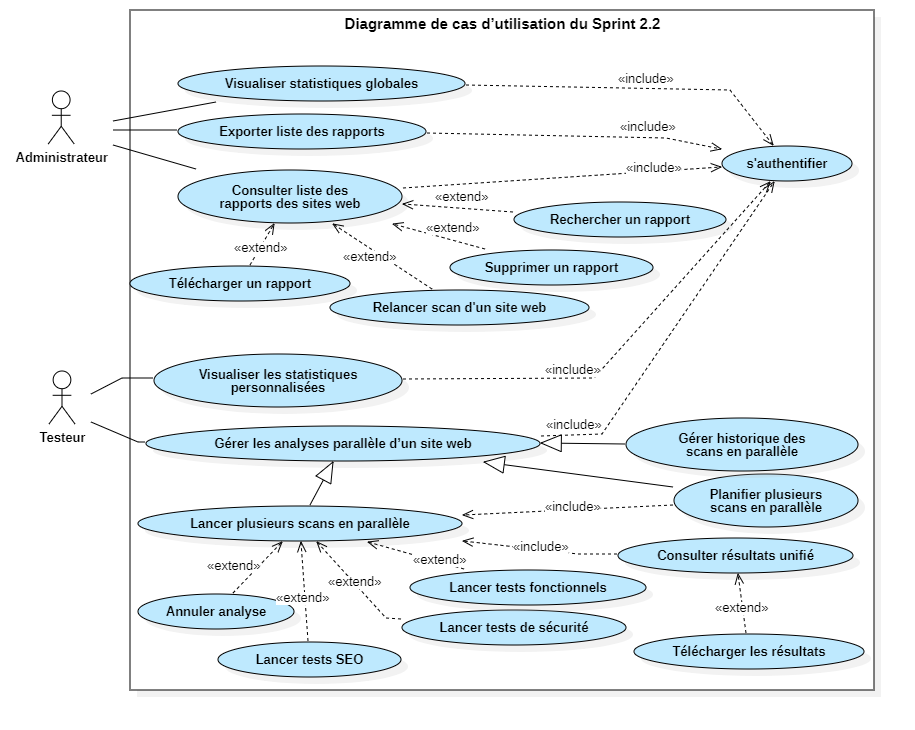
\includegraphics[width=\linewidth]{chapitres/ch4Sp2/section/sprint2.2/img/LastUseCaseSprint2.2.png}
    \caption{Diagramme de cas d'utilisation du sprint 2.2}
    \label{fig:caseS22}
\end{figure}
\vspace{-0.3cm}

